\documentclass[11pt,a4paper]{article}
\usepackage[utf8]{inputenc}
\usepackage[T1]{fontenc}
\usepackage{amsfonts}
\usepackage[french]{babel}
\frenchbsetup{StandardLists=true} % à inclure si on utilise \usepackage[francais]{babel}
\usepackage{enumitem}
\usepackage{amssymb}
\usepackage{amsmath}
\usepackage[left=2cm,right=2cm,top=2cm,bottom=2cm]{geometry}
\usepackage{multirow}
\usepackage[dvipsnames]{xcolor}

\usepackage[T1]{fontenc}
\usepackage{fouriernc}
\usepackage{graphicx}

\usepackage{setspace}
\singlespacing

\usepackage{pstricks}
\usepackage{xkeyval}
\usepackage{pst-labo}


\usepackage{multicol}
\usepackage{caption}
\usepackage{fancyhdr}
\pagestyle{fancy}
\renewcommand\headrulewidth{1pt}
\fancyhead[L]{Lycée Denis Diderot }
\fancyhead[R]{Classe de 1 Bac Pro }
\setcounter{page}{3}\fancyfoot[C]{page \thepage}
\fancyfoot[R]{Année 2024-2025}
\fancyfoot[L]{Alexis RUIZ}
\usepackage{multirow,tabularx,booktabs}
\usepackage[tikz]{bclogo} 

\newcommand{\cadreblanc}[1]{%
\medskip\framebox[\linewidth][c]{%
\rule{0mm}{#1mm}}\par
\medskip}

\usepackage{awesomebox}
\setlength{\aweboxvskip}{0mm}
\usepackage{pifont}
\usepackage{chemmacros}
\chemsetup{modules=all}
\setlength{\columnseprule}{.25mm}

\renewcommand{\arraystretch}{2.5}
\newcommand*\acocher{\quitvmode{\fboxsep0pt \fboxrule0.8pt \fbox{\vrule height1.8ex depth.1ex width0pt \vrule height0pt depth0pt width1.9ex }}}

\newcolumntype{C}[1]{>{\centering\arraybackslash }b{#1}}

\newcommand{\code}{\awesomebox[black]{2pt}{

\includegraphics[scale=0.15]{../Chapitre 1 - Energie et puissance électrique/images/frame.png}
}{black}}

\newcommand{\moteur}{\awesomebox[black]{2pt}{

\includegraphics[scale=1]{images/moteur.jpg} 
}{black}}

\newcommand{\defconclusion}{\awesomebox[black]{2pt}{\rotatebox{90}{\Large{\textbf{Conclusion}}}}{black}}

\newcommand{\defbox}{\awesomebox[black]{2pt}{
\includegraphics[scale=0.5]{../Chapitre 1 - Energie et puissance électrique/images/appel exam.png}}{black}}

  \newenvironment{itemize*}%  % listes compactes
    {\begin{itemize}%
      \setlength{\itemsep}{0pt}%
      \setlength{\parskip}{0pt}}%
    {\end{itemize}}

\frenchbsetup{StandardLists=true}



\usepackage[tikz]{bclogo} 
\newcommand{\ctext}[1]
{\begin{bclogo}[couleur = white,logo= , arrondi = 0.1,barre=none]
{}
\vspace{-8mm}
~~
\textcolor{black}{#1}
~~
\end{bclogo}}



\begin{document}

\flushleft \textbf{NOM : \hfill Classe : \hspace{3cm} ~~\\[2mm]
Prénom:\\[0,4cm]
}
\hrule\
\\[0,2cm]

\begin{center}
 \LARGE{TP1  - Le liquide magique  }


\vspace{3 mm}
\hrule


\normalsize
\end{center}

\ding{202}~~Réalisation du liquide magique \\ [3mm]

Lire la BD. Le Schtroumpf curieux fait appel à vous pour préparer le liquide magique.

\vfill 

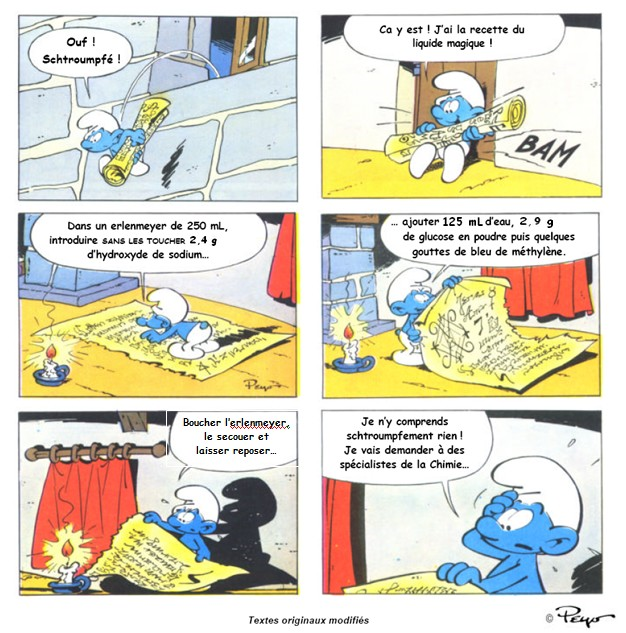
\includegraphics[scale=0.8]{images/BD.png}

\vfill 

\newpage

\ding{203}~~Retrouver le nom de chacun de ces instruments de chimie.\\[3mm]
\begin{center}
    
    \begin{tabular}{|C{3.2cm}|C{3.2cm}|C{3.2cm}|C{3.2cm}|} 
    \hline
       \psset{unit=0.5cm}
\pstTubeEssais[] & \psset{unit=0.5cm}\pstTubeEssais[glassType=erlen] & \psset{unit=0.5cm}\pstTubeEssais[glassType=becher] &  \psset{unit=0.5cm}\pstEprouvette\\
    \hline
         &  &  & \\
    \hline
    \end{tabular}
\end{center}




\ding{204}~~Réécrire la recette en précisant le mode opératoire. \\




    \ctext{Produits chimiques :
    \vspace{3cm 
    }}

    

    \ctext{Matériel necessaire :
    \vspace{3cm 
    }}

    

    \ctext{Protocole :
    \vspace{7cm 
    }}

\vfill 
    \defbox{\fbox{
\begin{minipage}{8cm}{

Appeler M Ruiz pour qu'il vérifie votre mode opératoire.}
\end{minipage}
}}

    \vfill 

    


\end{document}